\documentclass{tutorial}
\usepackage{tikz, tkz-berge}
\begin{document}
\newif\ifsolns

%%%%%%%%%%%%%%%%%%%%%%%%%
% UNCOMMENT BELOW TO TURN ON SOLNS %
%%%%%%%%%%%%%%%%%%%%%%%%%
\solnstrue

\title{EE241 Spring 2015: Tutorial \#3}
\date{Friday, Jan. 30, 2015}
\maketitle

%Graph connectivity
\begin{prob}
Consider the following graph representing the friendships of Franceska, Harry, Nicole, Bjork, and Sam.
\begin{center} 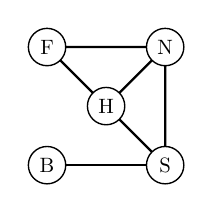
\begin{tikzpicture}[scale=0.75,transform shape]
  \Vertex[x=0,y=2] F
  \Vertex[x=1,y=1] H 
  \Vertex[x=0,y=0] B 
  \Vertex[x=2,y=2] N 
  \Vertex[x=2,y=0] S 
  \Edge (H)(S)
  \Edge (H)(N)
  \Edge (F)(H)
  \Edge (F)(N)
  \Edge (S)(B)
  \Edge (S)(N)
\end{tikzpicture} \end{center}
\begin{enumerate}[label=(\alph*)]
\item What is the adjacency matrix of this friend group? What do the entries represent?
\item What is the square of this matrix? What does it represent?
\item If any one member of this group wanted to notify all other members of a party via email, but they did not have the addresses of people they were not friends with, what is the maximum number of ``FWD:" would you expect to find in the subject line of the last person hearing about the party?
\end{enumerate}
\end{prob} \ifsolns \begin{proof}
\begin{enumerate}[label=(\alph*)]
\item The adjacency matrix is for $\ls F, H, N, B, S \rs$ is
\[
    A = \ls \begin{array}{ccccc}
        1 & 1 & 1 & 0 & 0 \\
        1 & 1 & 1 & 0 & 1 \\
        1 & 1 & 1 & 0 & 1 \\
        0 & 0 & 0 & 1 & 1 \\
        0 & 1 & 1 & 1 & 1 \\
    \end{array} \rs
\]
Note that we've used a different convention than the one in the notes for this matrix. We've added $1$'s on the diagonal. This can be interpretted as allowing for self-loops on each of the nodes of the graph. In other words, when traversing the graph above one can always choose to either stay put \emph{or} move to a connected node. Although this changes the graph fundamentally, it does not significantly affect our analysis in this question.
\item The square of this matrix is
\[
    A^2 = \ls \begin{array}{ccccc}
        3 & 3 & 3 & 0 & 2 \\
        3 & 4 & 4 & 1 & 3 \\
        3 & 4 & 4 & 1 & 3 \\
        0 & 1 & 1 & 2 & 2 \\
        2 & 3 & 3 & 2 & 4 \\
    \end{array} \rs
\]
The entries represent the number of paths that can take each column to each row in two steps (including staying put).
\item Here we just need to find a value $k$ such that $A^k$ has no non-zero entries. However, calculating $A^3$ by hand from the previous part might be a little too tedious (that is, only if you're doing these calculations in your head. On a computer there is no difference). Let's instead replace all the non-zero values in $A^2$ with $1$. At the graph level this is equivalent to forming connecting direct connections between all of the nodes that can be reached in two steps. This adjaceny matrix of the new graph is
\[
    \tilde{A} = \ls \begin{array}{ccccc}
        1 & 1 & 1 & 0 & 1 \\
        1 & 1 & 1 & 1 & 1 \\
        1 & 1 & 1 & 1 & 1 \\
        0 & 1 & 1 & 1 & 1 \\
        1 & 1 & 1 & 1 & 1 \\
    \end{array} \rs
\]
which indicates that $F$ is not connect to $B$ yet. In fact, this can be seen visually in the graph now updated with the new connections
\begin{center} 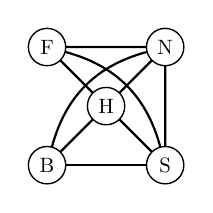
\begin{tikzpicture}[scale=0.75,transform shape]
  \Vertex[x=0,y=2] F
  \Vertex[x=1,y=1] H 
  \Vertex[x=0,y=0] B 
  \Vertex[x=2,y=2] N 
  \Vertex[x=2,y=0] S 
  \Edge (H)(S)
  \Edge (H)(N)
  \Edge (H)(B)
  \Edge (F)(H)
  \Edge (F)(N)
  \Edge (S)(B)
  \Edge (S)(N)
  \tikzstyle{EdgeStyle}=[bend left]
  \Edge (B)(N)
  \Edge (F)(S)
\end{tikzpicture} \end{center}
So, to find just the connectivity (and not necessarily the number of paths) that arises from allowing three steps on the graph, we can just calculate $A\tilde{A}$ which is
\[
    A\tilde{A} = \ls \begin{array}{ccccc}
        3 & 3 & 3 & 2 & 3 \\
        4 & 4 & 4 & 3 & 4 \\
        4 & 4 & 4 & 3 & 4 \\
        1 & 2 & 2 & 2 & 2 \\
        3 & 4 & 4 & 4 & 4 \\
    \end{array} \rs
\]
Note two important things: First, $A\tilde{A} \neq A^3$. Second, $A\tilde{A}$ has no zero entries. Thus, any two nodes of the graph can be reached in at most three steps and one would expect to find three ``FWD:" in the party invitation subject line.
\end{enumerate}
\end{proof}\else \newpage \fi

%Augmented matrix for solving equations (RREF) --> free vars, write soln as lin comb of vectors
  % Review that is called "Gauss-Jordan"
  % EVERY MATRIX is equivalent to exactly one other matrix in RREF (draw a many to one relationship, even though both sets are infinite)
\begin{prob}
Solve the following system using an augmented matrix and Gaussian elimination (get the matrix to reduced echelon form). Which variables are pivots? Which are free?
\[
    \ls \begin{array}{rrrrr}
         0 & 2 & 4 & 6 & 1 \\
        -1 & 0 & 0 & 1 &-1 \\
         0 & 1 & 2 & 3 & 1 \\
        -1 &-1 &-2 &-2 & 0 \\
    \end{array} \rs \vec{x}
     = \ls \begin{array}{r}
        1 \\ -1 \\ 1 \\ 0
     \end{array} \rs
\]
\end{prob} \ifsolns \begin{proof}
To solve this system we begin by writing down the augmented matrix $[A|\vec{b}]$
\[
    \ls \begin{array}{r|r} A & \vec{b} \end{array} \rs
    = \ls \begin{array}{rrrrr|r}
         0 & 2 & 4 & 6 & 1 & 1 \\
        -1 & 0 & 0 & 1 &-1 &-1 \\
         0 & 1 & 2 & 3 & 1 & 1 \\
        -1 &-1 &-2 &-2 & 0 & 0 \\
    \end{array} \rs
\]
To get the first pivot, we can multiply the second row by $-1$ and switch the first and second row
\[
    \ls \begin{array}{rrrrr|r}
         1 & 0 & 0 &-1 & 1 & 1 \\
         0 & 2 & 4 & 6 & 1 & 1 \\
         0 & 1 & 2 & 3 & 1 & 1 \\
        -1 &-1 &-2 &-2 & 0 & 0 \\
    \end{array} \rs
\]
We require that pivots are followed by zeros in their column and so we can add the first row \textbf{to} the four row
\[
    \ls \begin{array}{rrrrr|r}
         1 & 0 & 0 &-1 & 1 & 1 \\
         0 & 2 & 4 & 6 & 1 & 1 \\
         0 & 1 & 2 & 3 & 1 & 1 \\
         0 &-1 &-2 &-3 & 1 & 1 \\
    \end{array} \rs
\]
We now move to the second column to find the second pivot. Let's use row $3$ so that we don't get fractions (thankfully, we can use some freedom of choice here to keep the numbers a little cleaner). Let's switch rows $2$ and $3$
\[
    \ls \begin{array}{rrrrr|r}
         1 & 0 & 0 &-1 & 1 & 1 \\
         0 & 1 & 2 & 3 & 1 & 1 \\
         0 & 2 & 4 & 6 & 1 & 1 \\
         0 &-1 &-2 &-3 & 1 & 1 \\
    \end{array} \rs
\]
Now, in one step, let's add $-2$ of row $2$ to row $3$ and $1$ of row $2$ to row $4$
\[
    \ls \begin{array}{rrrrr|r}
         1 & 0 & 0 &-1 & 1 & 1 \\
         0 & 1 & 2 & 3 & 1 & 1 \\
         0 & 0 & 0 & 0 &-1 &-1 \\
         0 & 0 & 0 & 0 & 2 & 2 \\
    \end{array} \rs
\]
We notice that the third and fourth columns \emph{do not have pivots} so we skip them and move to column $5$. Here, let's multiply row $3$ by $-1$ and subtract twice row $3$ from row $4$
\[
    \ls \begin{array}{rrrrr|r}
         1 & 0 & 0 &-1 & 1 & 1 \\
         0 & 1 & 2 & 3 & 1 & 1 \\
         0 & 0 & 0 & 0 & 1 & 1 \\
         0 & 0 & 0 & 0 & 0 & 0 \\
    \end{array} \rs
\]
Since all rows are led by pivots or zeros and since each pivot is followed by zeros in its column, we have arrived at \emph{row echelon form}. We can now use back-substitution to find that
\[
    \lb \begin{array}{rl}
        x_5 & = 1 \\
        x_2 + 2x_3 + 3x_4 & = 0 \\
        x_1 - x_4 & = 0
    \end{array} \right.
\]
The pivot variables are $x_1$, $x_2$, and $x_5$. The free variables are $x_3$ and $x_4$. To write down the full set of solutions, let $x_3 = s$ and $x_4=t$ where $s,t \in \mbR$ and we can write
\[
    \vec{x} \in \lb \ls \begin{array}{c} t \\ -2s - 3t \\ s \\ t \\ 1 \end{array} \rs \; , \; \forall \; s,t \in \mbR \rb
\]
Or, equivalently, as a linear combination of vector with $s$ and $t$ as the coefficients we can write
\[
    \vec{x} \in \lb 
            \ls \begin{array}{r} 0 \\ 0 \\ 0 \\ 0 \\ 1 \end{array} \rs  
        + s \ls \begin{array}{r} 0 \\ -2 \\ 1 \\ 0 \\ 0 \end{array} \rs
        + t \ls \begin{array}{r} 1 \\ -3 \\ 0 \\ 1 \\ 0 \end{array} \rs
    \; , \; \forall \; s,t \in \mbR \rb
\]

\end{proof}\else \newpage \fi

%Particular and homogenous solutions (1 particular, 2-d homogenous)
  %Every solution to Ax=b can be written in this way
\begin{prob}
A mixture $5$ nuclear isotopes is being mixed into a fuel to be burned in $3$ different power plants. Each fuel burns at a different temperature in each plant and each plant can only tolerate a certain amount of heat. Since the tolerances and the burning temperatures are top-secret they are not known to the public. You are asked by the department of energy to find all suitable mixtures of isotopes. You are given only the following information: The department of energy once developed a suitable fuel once with the following ratios $\ls 0.2, 0.1, 0.4, 0.1, 0.2 \rs$ and the matrix $A$ which converts isotope to temperature has the following row-reduced echelon form
\[
    \ls \begin{array}{rrrrr}
        1 & -0.2 & 0 & -0.4 & -0.1 \\
        0 &    0 & 1 & -0.5 & -0.2 \\
        0 &    0 & 0 &    0 &    0 \\
    \end{array} \rs
\]
Find the set of all suitable isotope mixtures.
\end{prob} \ifsolns \begin{proof}
First, we know that $A \vec{x}_p = \vec{b}$. We now need to find only the homogenous solutions. Since there are $3$ free variables in the rref of $A$, we will have a set with three free variables. Let $x_2 = s$, $x_4 = t$, and $x_5 = u$. Then we have that any homogenous solution is given by
\[
    \vec{x}_h \in \lb 
          s \ls \begin{array}{r} 0.2 \\ 1 \\ 0   \\ 0 \\ 0 \end{array} \rs
        + t \ls \begin{array}{r} 0.4 \\ 0 \\ 0.5 \\ 1 \\ 0 \end{array} \rs
        + u \ls \begin{array}{r} 0.1 \\ 0 \\ 0.2 \\ 0 \\ 1 \end{array} \rs
    \; , \; \forall \; s,t,u \geq 0 \rb
\]
Altogether, the suitable isotope mixtures are
\[
    \vec{x} \in \lb 
            \ls \begin{array}{r} 0.2 \\ 0.1 \\ 0.4 \\ 0.1 \\ 0.2 \end{array} \rs
        + s \ls \begin{array}{r} 0.2 \\   1 \\ 0   \\ 0   \\ 0   \end{array} \rs
        + t \ls \begin{array}{r} 0.4 \\   0 \\ 0.5 \\ 1   \\ 0   \end{array} \rs
        + u \ls \begin{array}{r} 0.1 \\   0 \\ 0.2 \\ 0   \\ 1   \end{array} \rs
    \; , \; \forall \; s,t,u \geq 0 \rb
\]
(note that technically, we should ensure that the proportions add to $1$ but we'll ignore that fact for now)
\end{proof}\else \newpage \fi

%Particular and homogenous solutions (1 particular, 1-d homogenous)
\begin{prob}
Powell who is hosting the party from question (1) has the email addresses of everyone involved. He would like to update everyone in the group on the party's location but doesn't want anyone receiving multiple copies of the message for fear of annoying them (Powell needs to chill out). He knows that whoever he sends an email to directly will then forward that email to everyone they know. Who should he send emails to so that everyone gets the message only once? If Powell can send negative emails (e.g.: apologies), what other configurations are there?
\end{prob} \ifsolns \begin{proof}
If we let $\vec{x}$ be a vector of the number of emails Powell sends to each of the group members then the system we are trying to solve is
\[
    A \vec{x} = \ls \begin{array}{c} 1 \\ 1 \\ 1 \\ 1 \\ 1 \end{array} \rs
\]
Let's proceed with Gaussian elimination on the augmented matrix
\[
    \ls \begin{array}{rrrrr|r}
        1 & 1 & 1 & 0 & 0 & 1 \\
        1 & 1 & 1 & 0 & 1 & 1 \\
        1 & 1 & 1 & 0 & 1 & 1 \\
        0 & 0 & 0 & 1 & 1 & 1 \\
        0 & 1 & 1 & 1 & 1 & 1
    \end{array} \rs
    \hspace{0.15in} \Longrightarrow \hspace{0.15in}
    \ls \begin{array}{rrrrr|r}
        1 & 1 & 1 & 0 & 0 & 1 \\
        0 & 0 & 0 & 0 & 1 & 0 \\
        0 & 0 & 0 & 0 & 1 & 0 \\
        0 & 0 & 0 & 1 & 1 & 1 \\
        0 & 1 & 1 & 1 & 1 & 1
    \end{array} \rs
\]
\[
    \ls \begin{array}{rrrrr|r}
        1 & 1 & 1 & 0 & 0 & 1 \\
        0 & 1 & 1 & 1 & 1 & 1 \\
        0 & 0 & 0 & 1 & 1 & 1 \\
        0 & 0 & 0 & 0 & 1 & 0 \\
        0 & 0 & 0 & 0 & 1 & 0 \\
    \end{array} \rs
    \hspace{0.15in} \Longrightarrow \hspace{0.15in}
    \ls \begin{array}{rrrrr|r}
        1 & 1 & 1 & 0 & 0 & 1 \\
        0 & 1 & 1 & 1 & 0 & 1 \\
        0 & 0 & 0 & 1 & 0 & 1 \\
        0 & 0 & 0 & 0 & 1 & 0 \\
        0 & 0 & 0 & 0 & 0 & 0 \\
    \end{array} \rs
\]
\[
    \ls \begin{array}{rrrrr|r}
        1 & 1 & 1 & 0 & 0 & 1 \\
        0 & 1 & 1 & 0 & 0 & 0 \\
        0 & 0 & 0 & 1 & 0 & 1 \\
        0 & 0 & 0 & 0 & 1 & 0 \\
        0 & 0 & 0 & 0 & 0 & 0 \\
    \end{array} \rs
    \hspace{0.15in} \Longrightarrow \hspace{0.15in}
    \ls \begin{array}{rrrrr|r}
        1 & 0 & 0 & 0 & 0 & 1 \\
        0 & 1 & 1 & 0 & 0 & 0 \\
        0 & 0 & 0 & 1 & 0 & 1 \\
        0 & 0 & 0 & 0 & 1 & 0 \\
        0 & 0 & 0 & 0 & 0 & 0 \\
    \end{array} \rs
\]
Thus, the solution is for Powell to send one email to Franceska ($x_1 = 1$) and one email to Bjork ($x_4=1$). However! If Powell is also allowed to send apologies (negative emails) then he could also send one email to Harry ($x_2=1$) so long as he also sent an apology to Nicole ($x_3=-1$). This can be seen from the decomposition of the solution into the particular and homogenous parts as
\[
    \vec{x} \in \lb 
            \ls \begin{array}{r} 1 \\ 0 \\ 0 \\ 1 \\ 0 \end{array} \rs
        + s \ls \begin{array}{r} 0 \\-1 \\ 1 \\ 0 \\ 0 \end{array} \rs
    \; , \; \forall s \in \mbZ
    \rb
\]
\end{proof}\else \newpage \fi


\end{document}